\documentclass[11pt,letterpaper]{article}

\usepackage[margin=1in]{geometry}
\usepackage{graphicx}
\usepackage{subcaption}
\usepackage{booktabs}
\usepackage{hyperref}
\usepackage{parskip}
\usepackage{float}
\usepackage{microtype}
\usepackage{soul}
\usepackage{amsmath}

\hypersetup{colorlinks=true, linkcolor=blue, urlcolor=blue}

\title{\textbf{CS5330 Computer Vision: Project 3}\\
       \large Real-Time 2-D Object Recognition}
\author{Shriman Raghav Srinivasan \and Shyam Sreenivasan}
\date{June 2026}

\begin{document}

\maketitle

% ============================================================
\section*{Project Overview}
% ============================================================

In this project, we developed a computer vision system to recognize 2D objects in real time. The system processes video frames from a live camera feed or static images. It isolates candidate objects, cleans up image noise, segments regions, computes shape features, and classifies the objects.

All core image processing steps are written from scratch without using OpenCV's high-level functions. We implemented our own thresholding, morphological filters, connected components finder, and moment-based feature extraction.

We divided the work. Shriman Raghav Srinivasan implemented Tasks 1 through 4 (preprocessing, segmentation, and OBB feature extraction) and Task 9 (deep network embedding classification). Teammate Shyam Sreenivasan is responsible for implementing Tasks 5 through 7 (collecting training data and implementing the classical standardized distance classifier).

% ============================================================
\section*{Source Code}
% ============================================================

The full source code for this project is available at:\\
\url{https://github.com/shyams612/CS5330-Computer-Vision/tree/main/Projects/project3}

Instructions for building and running the code are provided in the repository's \texttt{README.md}.

% ============================================================
\section*{Methodology and Results}
% ============================================================

%------------------------------------------------------------
\subsection*{Task 1, 2, and 3: Preprocessing and Segmentation}
%------------------------------------------------------------

First, we apply a 3x3 box blur filter to reduce high-frequency noise. We then convert the image to binary. We support two thresholding modes: manual and dynamic. The dynamic mode uses the iterative ISODATA method. This algorithm finds a threshold that separates the foreground and background by averaging their mean values. The thresholding step also supports inverting the binary mask.

Next, we clean up the binary mask using morphological operations. We implemented erosion and dilation from scratch using pixel loops. We combine these into opening and closing operations. Opening removes small isolated noise pixels. Closing fills in internal holes.

Finally, we segment the cleaned mask into regions. We implemented a queue-based 8-connected flood fill. The algorithm labels every foreground pixel with a unique region ID. We prune regions smaller than 500 pixels to eliminate noise.

Figures~\ref{fig:preprocessing} show the steps of this pipeline on the first development image.

\begin{figure}[H]
    \centering
    \begin{subfigure}[b]{0.23\textwidth}
        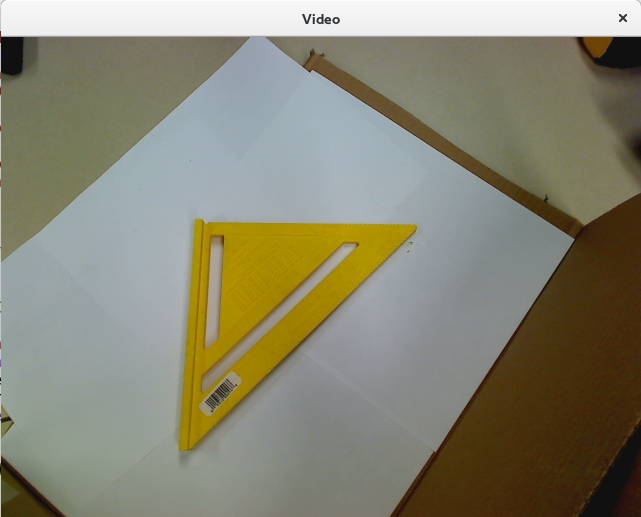
\includegraphics[width=\textwidth]{report_imgs/orig_dev1.png}
        \caption{Original Image}
    \end{subfigure}
    \hfill
    \begin{subfigure}[b]{0.23\textwidth}
        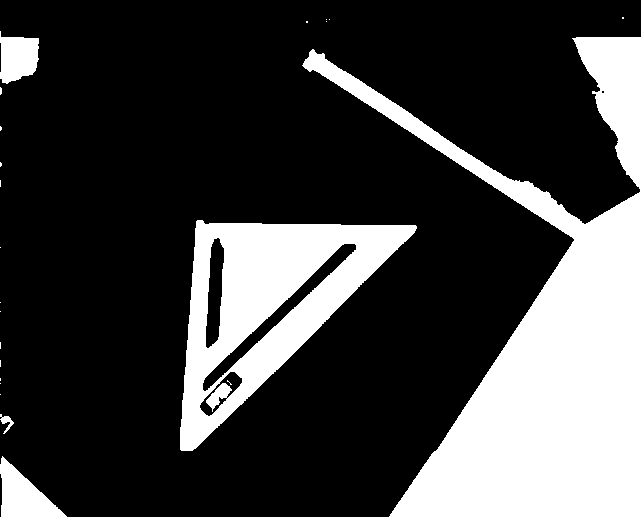
\includegraphics[width=\textwidth]{report_imgs/thresh_dev1.png}
        \caption{Binary Mask}
    \end{subfigure}
    \hfill
    \begin{subfigure}[b]{0.23\textwidth}
        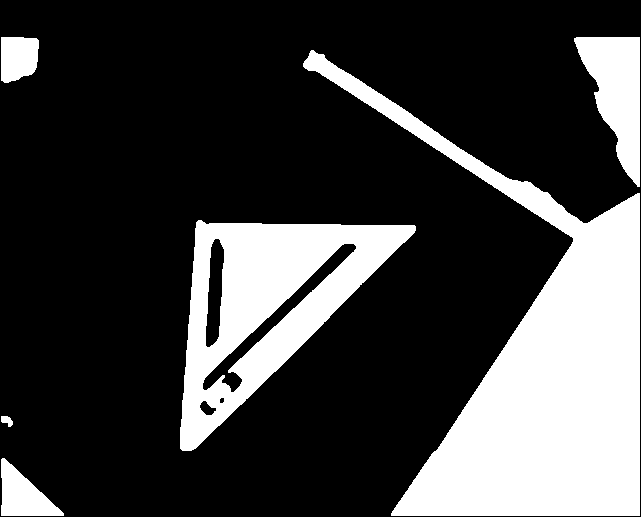
\includegraphics[width=\textwidth]{report_imgs/clean_dev1.png}
        \caption{Cleaned Mask}
    \end{subfigure}
    \hfill
    \begin{subfigure}[b]{0.23\textwidth}
        
\includegraphics[width=\textwidth]{report_imgs/regions_dev1.png}
        \caption{Regions Map}
    \end{subfigure}
    \caption{Preprocessing and segmentation stages for \texttt{img1p3.png}. The custom morphological filter removes stray noise and closes internal holes. The connected components finder then segments the objects.}
    \label{fig:preprocessing}
\end{figure}

%------------------------------------------------------------
\subsection*{Task 4: Feature Extraction and Bounding Boxes}
%------------------------------------------------------------

For each segmented region, we compute its moments to extract shape descriptors. We calculate the centroid coordinates ($\bar{x}, \bar{y}$) and the central moments ($\mu_{20}, \mu_{02}, \mu_{11}$). 

Using these central moments, we calculate the primary orientation angle ($\theta$):
\[
\theta = \frac{1}{2} \arctan\left(\frac{2\mu_{11}}{\mu_{20} - \mu_{02}}\right)
\]
We also compute elongation by finding the eigenvalues of the covariance tensor, taking the ratio of the maximum eigenvalue to the minimum eigenvalue.

To compute the Oriented Bounding Box (OBB), we project each pixel coordinate in a region onto the primary axis ($\vec{e}_1$) and secondary axis ($\vec{e}_2$) relative to the centroid:
\[
p_1 = (c - \bar{x})\cos\theta + (r - \bar{y})\sin\theta
\]
\[
p_2 = -(c - \bar{x})\sin\theta + (r - \bar{y})\cos\theta
\]
We find the minimum and maximum projection values ($minE_1, maxE_1, minE_2, maxE_2$) for each region. These values represent the bounding box extents. We render the OBB by rotating the corners back to original image coordinates and drawing green lines.

Table~\ref{tab:features} details the computed features for all segmented regions in the 5 development images. Figure~\ref{fig:features} shows the OBB overlays for development images 1 and 2.

\begin{table}[H]
\centering
\small
\begin{tabular}{ccccccc}
\toprule
Image & Region & Centroid ($x, y$) & Elongation & Orient (deg) & Extent 1 ($min, max$) & Extent 2 ($min, max$) \\
\midrule
Img 1 & 1 & (17.896, 57.291) & 1.518 & -66.472 & [-28.202, 24.914] & [-23.592, 20.474] \\
Img 1 & 2 & (616.989, 91.550) & 8.426 & 77.538 & [-62.109, 96.975] & [-33.263, 31.068] \\
Img 1 & 3 & (543.214, 369.967) & 2.631 & 82.722 & [-346.808, 155.999] & [-117.434, 199.769] \\
Img 1 & 4 & (267.233, 302.391) & 3.353 & -46.591 & [-165.806, 157.080] & [-106.993, 58.248] \\
Img 1 & 5 & (22.700, 495.221) & 2.985 & 41.355 & [-40.221, 43.319] & [-15.705, 29.184] \\
\midrule
Img 2 & 1 & (85.862, 113.372) & 2.969 & -39.134 & [-154.922, 171.154] & [-111.392, 63.178] \\
Img 2 & 2 & (498.931, 283.002) & 2.138 & -81.024 & [-263.939, 264.843] & [-303.270, 176.527] \\
Img 2 & 3 & (33.582, 493.627) & 3.721 & 24.574 & [-44.369, 72.019] & [-23.242, 32.571] \\
\midrule
Img 3 & 1 & (83.982, 113.956) & 2.967 & -40.123 & [-154.106, 168.369] & [-110.148, 61.318] \\
Img 3 & 2 & (522.118, 275.830) & 3.590 & 89.706 & [-238.237, 241.771] & [-119.099, 258.345] \\
Img 3 & 3 & (280.222, 334.790) & 37.298 & 26.376 & [-85.949, 60.342] & [-26.362, 12.066] \\
Img 3 & 4 & (38.181, 495.148) & 4.514 & 21.055 & [-47.829, 80.330] & [-25.547, 32.673] \\
\midrule
Img 4 & 1 & (525.334, 271.570) & 3.846 & 87.682 & [-243.382, 248.747] & [-122.979, 263.972] \\
Img 4 & 2 & (83.467, 113.075) & 2.958 & -39.585 & [-155.268, 169.247] & [-110.409, 61.509] \\
Img 4 & 3 & (288.500, 367.683) & 53.922 & -50.137 & [-102.216, 172.290] & [-25.194, 22.427] \\
Img 4 & 4 & (31.708, 493.973) & 3.347 & 26.551 & [-45.337, 66.910] & [-23.372, 33.430] \\
\midrule
Img 5 & 1 & (83.526, 113.879) & 2.910 & -40.157 & [-155.370, 169.168] & [-111.213, 62.113] \\
Img 5 & 2 & (520.746, 273.419) & 3.558 & 89.215 & [-238.775, 243.178] & [-121.452, 262.030] \\
Img 5 & 3 & (283.751, 329.260) & 2.299 & -56.056 & [-53.728, 54.166] & [-34.590, 33.947] \\
Img 5 & 4 & (34.621, 493.549) & 4.121 & 23.250 & [-46.502, 74.050] & [-24.277, 32.981] \\
\bottomrule
\end{tabular}
\caption{Computed moments and OBB features for all segmented regions in the 5 development images.}
\label{tab:features}
\end{table}

\begin{figure}[H]
    \centering
    \begin{subfigure}[b]{0.48\textwidth}
        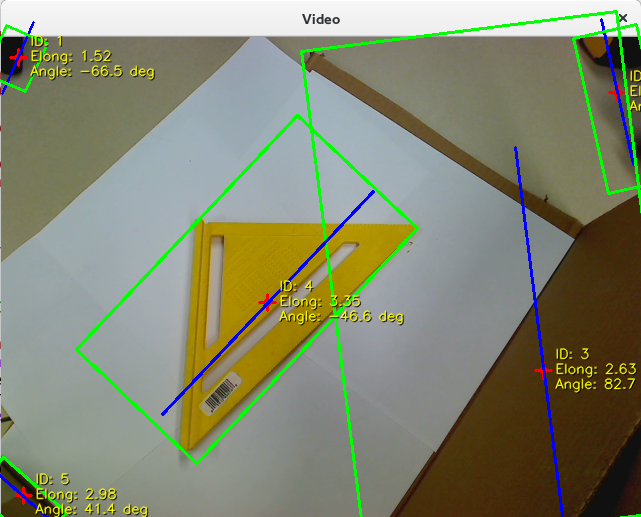
\includegraphics[width=\textwidth]{report_imgs/features_dev1.png}
        \caption{Dev Image 1}
    \end{subfigure}
    \hfill
    \begin{subfigure}[b]{0.48\textwidth}
        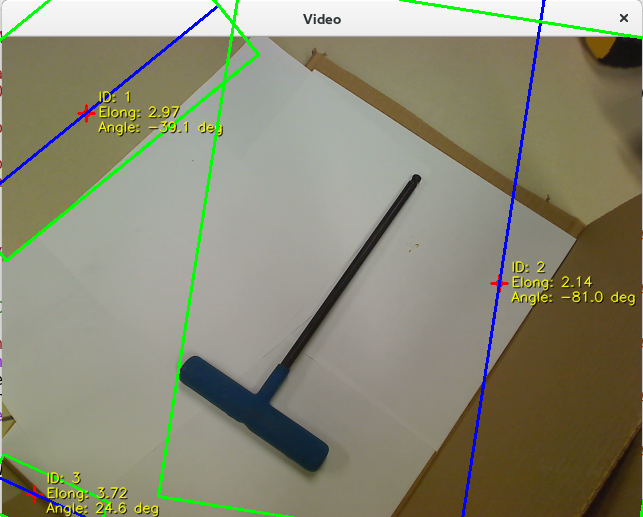
\includegraphics[width=\textwidth]{report_imgs/features_dev2.png}
        \caption{Dev Image 2}
    \end{subfigure}
    \caption{Visual overlays representing centroids (red dots), orientation axes (blue lines), statistics, and green Oriented Bounding Boxes (OBB) drawn around segmented objects.}
    \label{fig:features}
\end{figure}

%------------------------------------------------------------
\subsection*{Task 9: ResNet18 DNN Embedding Classifier}
%------------------------------------------------------------

We implemented a deep learning-based embedding classifier. The system extracts a feature vector from each segmented region using a pre-trained ResNet18 ONNX model.

First, we prepare the region image by rotating the original frame around the centroid by $-\theta$ degrees. This aligns the primary orientation axis horizontally. We crop the region using the OBB bounds and resize the crop to $224 \times 224$. We then pass this cropped ROI through the ResNet18 network using OpenCV's DNN module to extract a 512-dimensional embedding vector.

We implement a 1-NN classifier using cosine distance:
\[
D(A, B) = 1 - \frac{\vec{A} \cdot \vec{B}}{\|\vec{A}\|_2 \|\vec{B}\|_2}
\]
The system reads known embeddings from \texttt{saved\_thresholds/embeddings\_database.csv}. If the database is loaded, the classifier calculates the cosine distance to all entries and labels the object with the nearest class.

To train new objects, the user presses key \texttt{'e'}. The system freezes the feed and prompts for a class label in the display window. The user types the label and presses Enter. The system saves the embedding of the largest region to the database.

% ============================================================
\section*{Reflection}
% ============================================================

Implementing the morphological filter and region segmentation from scratch helped us understand the underlying mechanics of connected components. In Task 4, calculating the OBB required careful handling of coordinate frame rotations. Aligning the primary axis before cropping ensures scale and rotation invariance. The ResNet18 DNN embeddings proved highly robust. They represent semantic properties of objects, making them more resilient to minor thresholding defects than classical features.

% ============================================================
\section*{Acknowledgements}
% ============================================================

\begin{itemize}
    \item OpenCV documentation (\url{https://docs.opencv.org/4.x/}) for DNN loading and affine warping functions.
    \item Shriman Raghav Srinivasan implemented Tasks 1 through 4 (thresholding, morphology, segmentation, features, and OBB calculations) and Task 9 (deep network embedding classifier, cosine distance, and database integration).
    \item Teammate Shyam Sreenivasan will implement Tasks 5, 6, and 7 (training database and standardized Euclidean distance matching).
\end{itemize}

\end{document}
